\documentclass{mwart}
\usepackage[utf8]{inputenc}
\usepackage{indentfirst}
\usepackage{polski}
\usepackage{float}
\usepackage{hyperref}
\usepackage{amsmath}
\usepackage{xcolor}
\usepackage{listings}
\usepackage[caption = false]{subfig}
\usepackage[final]{graphicx}
\usepackage[a4paper, total={6in, 8in}]{geometry}

\usepackage{xcolor}
\usepackage{listings}
\usepackage{longtable}
\usepackage{natbib}
\usepackage{graphicx}

\definecolor{mGreen}{rgb}{0,0.6,0}
\definecolor{mGray}{rgb}{0.5,0.5,0.5}
\definecolor{mPurple}{rgb}{0.58,0,0.82}
\definecolor{backgroundColour}{rgb}{0.95,0.95,0.92}
\lstdefinestyle{JavaStyle}{
    backgroundcolor=\color{backgroundColour},   
    commentstyle=\color{mGreen},
    keywordstyle=\color{magenta},
    numberstyle=\tiny\color{mGray},
    stringstyle=\color{mPurple},
    basicstyle=\footnotesize,
    breakatwhitespace=false,         
    breaklines=true,                 
    captionpos=b,                    
    keepspaces=true,                 
    numbers=left,                    
    numbersep=5pt,                  
    showspaces=false,                
    showstringspaces=false,
    showtabs=false,                  
    tabsize=2,
    language=Java
}

\title{
    \textbf{Algorytmy ewolucyjne i metaheurystyki}\\ 
    \begin{large} 
        Sprawozdanie 1
    \end{large}
}

\author{
    Górka Bartosz\\
  \texttt{127228}
  \and
  Kajetan Zimniak\\
  \texttt{127229}
}

\date{}
\begin{document}

\maketitle

\section{Opis problemu}
Celem projektu było przygotowanie dwóch wersji algorytmów rozwiązujących problem grupowania. Liczba grup została ustalona na $10$. Funkcja celu to minimalizacja sumy długości minimalnych drzew rozpinających (minimum spanning tree) dla poszczególnych grup.

Jako kluczowe było wykorzystanie macierzy odległości (dystansu pomiędzy punktami) zamiast użycia przestrzeni kartezjańskiej jako punktu wyjścia. Takie założenie pozwala wykorzystać algorytmy również w przypadku zmiany funkcji odległości (macierz odległości jest wystarczająca do dokonania przydziału).

\section{Pseudokody przygotowanych algorytmów}
\subsection{Algorytm zachłanny}
Algorytm zachłanny dokonuje przydziału obiektu zgodnie z pseudokodem zaprezentowanym poniżej. Dla każdego punktu wybiera grupę do której ma najmniejszą wartość odległości (pomiędzy obecnym punktem a punktem startowym grupy). Po wybraniu najlepszego przydziału (najmniejsza odległość), dodajemy punkt do listy punktów przynależących do wybranej grupy.

\begin{lstlisting}[style=JavaStyle]
for each point in list of points {
    int pointID = point.getPointID();
    int selectedGroupID;
    double minDistance = Double.Max_Value;

    for each groupIndex in groups groups {
        double distance = distanceMatrix[groupIndex][pointID];
        
        if (distance < minDistance) {
            minDistance = distance;
            selectedGroupID = groupIndex;
        }
    }

    pointsInGroup[selectedGroupID].add(point);
}
\end{lstlisting}

\subsection{Algorytm z wykorzystaniem żalu}
TODO

\begin{lstlisting}[style=JavaStyle]
TODO
\end{lstlisting}

\section{Wyniki eksperymentów obliczeniowych}
W tabeli \ref{table:wyniki} zaprezentowano wyniki eksperymentów obliczeniowych. Dokonano $100$ powtórzeń obliczeń, za każdym razem z losowym wyborem elementu startowego w każdej z $10$ grup. Obydwa algorytmy wykorzystywały te same punkty startowe w ramach pojedynczej iteracji.

\begin{table}[H]
\centering
\caption{Wyniki eksperymentów obliczeniowych dla 100 iteracji}
\label{table:wyniki}
\resizebox{\textwidth}{!}{%
\begin{tabular}{|c|r|r|}
\hline
\textbf{Cecha}                                                                     & \multicolumn{1}{c|}{\textbf{Algorytm zachłanny}} & \multicolumn{1}{c|}{\textbf{Algorytm oparty o żal}} \\ \hline
\textbf{\begin{tabular}[c]{@{}c@{}}Wartość minimalna\\ funkcji celu\end{tabular}}  &                                                  &                                                     \\ \hline
\textbf{\begin{tabular}[c]{@{}c@{}}Wartość maksymalna\\ funkcji celu\end{tabular}} &                                                  &                                                     \\ \hline
\textbf{\begin{tabular}[c]{@{}c@{}}Wartość średnia\\ funkcji celu\end{tabular}}    &                                                  &                                                     \\ \hline
\textbf{\begin{tabular}[c]{@{}c@{}}Czas trwania\\ obliczeń {[}sec{]}\end{tabular}} &                                                  &                                                     \\ \hline
\end{tabular}%
}
\end{table}

TODO WNIOSKI
TODO dodać opis algorytmu z rozpiniem drzewa i usuwaniem krawędzi

\section{Wizualizacja najlepszych rozwiązań}
\subsection{Algorytm zachłanny}
\begin{figure}[H]
    \centering
    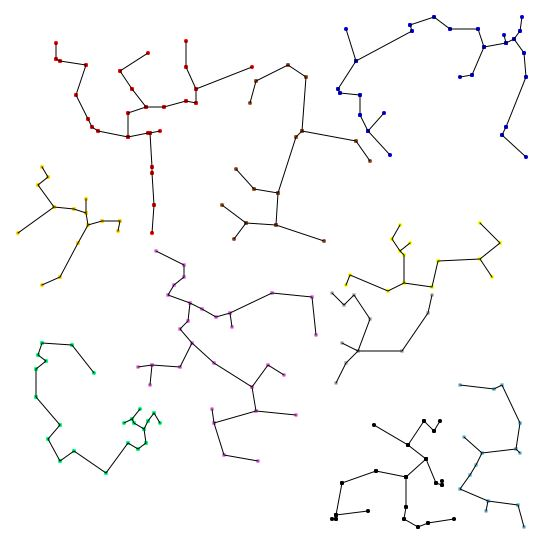
\includegraphics[width=\textwidth]{zachlanny.png}
    \caption{Algorytm zachłanny - wizualizacja najlepszego przydziału}
\end{figure}

\subsection{Algorytm oparty o żal}
\begin{figure}[H]
    \centering
    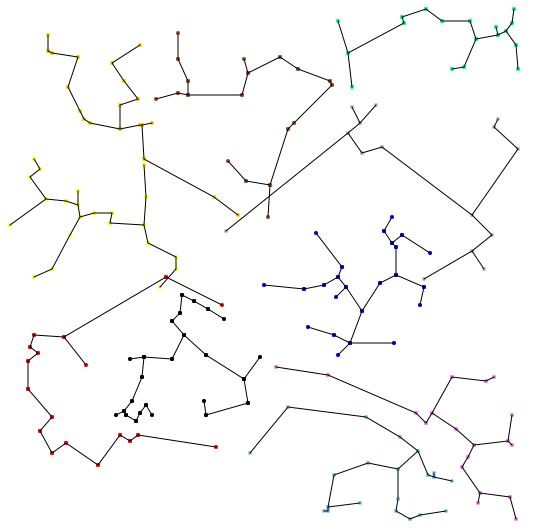
\includegraphics[width=\textwidth]{regret.png}
    \caption{Algorytm oparty o żal - wizualizacja najlepszego przydziału}
\end{figure}

\end{document}
